\clearpage
\section{Oligopol (charakteristiky, typy oligopolů, rovnováha oligopolu s dominantní firmou)}

\subsection{Charakteristiky oligopolu}
\begin{itemize}
    \item Existuje několik firem
    \item Diferencovaný produkt (zpravidla)
    \item Bariéry vstupu na trh
\end{itemize}

\subsection{Typy oligopolů}
\begin{itemize}
    \item Smluvní - firmy prodávají stejné nebo velmi podobné statky, tajné dohody o cenách na trhu. Kartelové dohody ale jsou v rozporu se zákonem.
    \item Oligopol s dominantní firmou - Dominantní firma přenechá část trhu menším firmám, ty přejímají cenu dominantní firmy
\end{itemize}

\subsection{Rovnováha oligopolu s dominantní firmou}
\begin{itemize}
    \item Pro dominantní firmu platí, že vyrábí takové množství, aby $MC_D=MR_D$, ale cenu udává podle svojí nabídkové křivky při tomto objemu. (tzv. \uv{cenové vůdcovství})
    \item Na trhu jsou 2 křivky poptávky; poptávka dominantní firmy a poptávka ostatních firem. Ostatní firmy přebírají cenu a vyrobené množství určují podle této ceny a svojí nabídkové křivky.
\end{itemize}
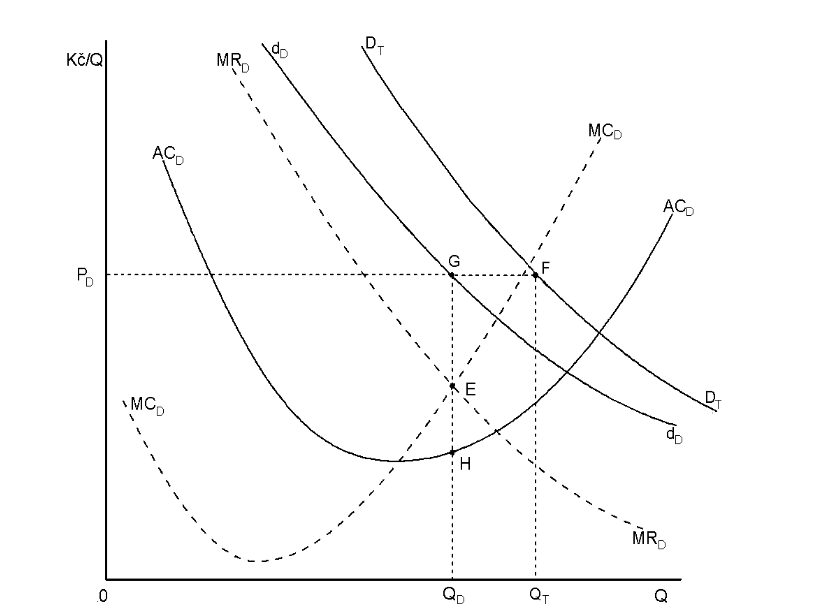
\includegraphics[width=16cm]{images/14_rovnovaha.png}